La conception de ce sprint commence par la présentation du diagramme de classes, représentant la structure du système.
\subsubsection{Diagramme de classe du sprint 1.1}
La figure \ref{fig:classsp1} illustre le diagramme de classes du sprint 1.1, représentant les principales entités métier, leurs attributs, leurs méthodes, ainsi que les relations entre elles.
\begin{figure}[H]
    \centering
    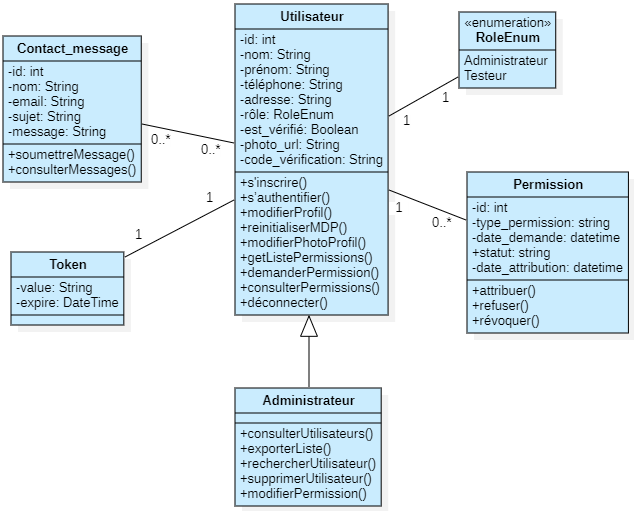
\includegraphics[width=0.9\linewidth]{chapitres/ch3Sp1/section/sprint1/img/classeL1-SP1.1.png}
    \caption{Diagramme de classe du sprint 1.1}
    \label{fig:classsp1}
\end{figure}
\vspace{-0.4cm}
Les principales classes modélisées de sprint 1.1 sont les suivantes:
    \begin{itemize}[label=$*$]
       \item \textbf{Utilisateur :} Représente les comptes utilisateurs de l’application. Elle contient des informations personnelles (nom, prénom, téléphone, adresse, email, mot de passe, et rôle (\texttt{RoleEnum}) ainsi que des méthodes relatives à la gestion du compte et d’administration des utilisateurs.
       \item \textbf{Contact\_message :} Permet aux utilisateurs de soumettre des messages via un formulaire de contact. Elle comprend des attributs et des méthodes pour stocker les détails du message.
       \item \textbf{RoleEnum (énumération) :} Définit les différents rôles possibles dans l’application, notamment \textit{Administrateur} et \textit{Testeur}, utilisés pour la gestion des droits d’accès.
       \item \textbf{Permission :} Représente les permissions associées aux utilisateurs, avec les attributs suivants : type de permission, date de demande, date d’attribution, statut, ainsi que les méthodes : révoquer, attribuer et refuser une demande de permission.
       \item \textbf{Token :} Modélise un jeton d’authentification, avec ses valeurs et sa date d’expiration, utilisé pour la gestion des sessions utilisateurs.
       \item \textbf{Administrateur :} Hérite de la classe Utilisateur et dispose de méthodes spécifiques pour la gestion des utilisateurs, comme consulter la liste des utilisateurs, rechercher, modifier leurs permissions, supprimer des utilisateurs, et exporter la liste.
    \end{itemize}
Les associations entre classes sont également représentées dans le diagramme, notamment:
\begin{itemize}[label=$-$, left=0.05cm]
    \item Un \texttt{Utilisateur} possède un rôle défini par \texttt{RoleEnum} et peut avoir plusieurs \texttt{Permission}.
    \item Un \texttt{Administrateur} : utilisateur disposant de privilèges étendus pour la gestion des autres comptes.
    \item Un \texttt{Utilisateur} peut générer un ou plusieurs \texttt{Token} pour gérer ses sessions.
    \item Un \texttt{Utilisateur} peut envoyer un \texttt{Contact\_message} à plusieurs administrateurs, tandis qu’un \texttt{Administrateur} peut recevoir des messages envoyés par plusieurs utilisateurs.
\end{itemize}
Ce diagramme constitue une base essentielle pour la suite du développement, en assurant une structure cohérente et maintenable du code tout au long des itérations agiles.
